%*----------- SLIDE -------------------------------------------------------------
\begin{frame}[t]{A Álgebra Linear} 

 É uma área da matemática que que permite estudos matemáticos mais aprofundados e soluções em aplicações práticas em diversos campos da ciência e negócios.
 \nocite{baldin2011geometria}\nocite{boldrini1980algebra}\nocite{craig2012robotica}

 \vspace*{0.8cm}

\begin{figure}
    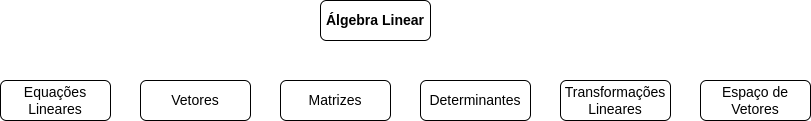
\includegraphics[width=\textwidth]{intro2.png}
\end{figure}
            
    \note[item]{Notes can help you to remember important information. Turn on the notes option.}
\end{frame}
%-

%*----------- SLIDE -------------------------------------------------------------
\begin{frame}[t]{Matriz e Vetores} 
    \begin{columns}
        \column{.01\textwidth}
        \column{.50\textwidth}
        \begin{itemize}
            \item Permitem escrever sistemas lineares de uma forma mais compacta
            \item E, utilizar operações com as matrizes para solucionar o sistema.
        \end{itemize}
        \column{.5\textwidth}
        \begin{figure}
            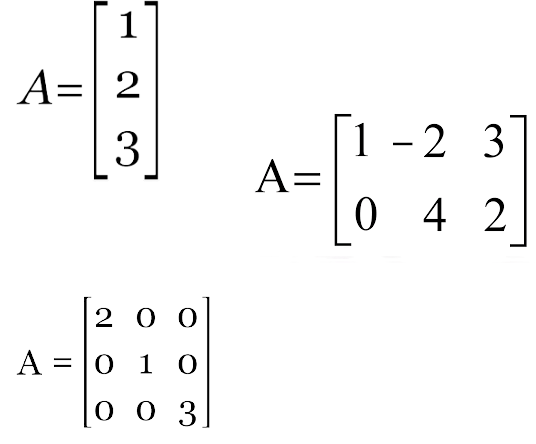
\includegraphics[width=0.8\textwidth]{matriz.png}
        \end{figure}
    \end{columns}
%*----------- notes
    \note[item]{Notes can help you to remember important information. Turn on the notes option.}
\end{frame}
%-